% Requires graphicx. Keep the figure PDF beside this fragment, or adjust its path.
% Use subsection here only if the surrounding manuscript already contains Introduction.
\subsection{Our Work}
\label{sec:our-work}

We develop a quality-aware routing and carbon-aware scheduling framework for SWITCH. Figure~\ref{fig:our-work} summarizes four linked stages of our work.

First, we combine public benchmarks, workload traces, energy evidence and grid-carbon data to evaluate response quality, inference cost, latency and emissions. Pre-inference quality prediction and post-response assessment provide complementary evidence for comparing routing policies.

Second, we compare direct and sequential-cascade policies under quality and cost constraints. The selected Pre-LightGBM router uses task-specific finite-sample risk guards and fallback to the more capable model; post-response escalation is not activated in the selected policy.

Third, we keep model choices fixed and formulate regional allocation as a Spatial MILP, with execution evaluated through discrete-event simulation. Comparisons with Greedy and temporal scheduling alternatives examine the trade-offs among carbon emissions, tail latency and service violations.

Finally, we assess robustness under task-mix shifts, prediction noise and demand growth, and examine fairness across request categories, rebound effects and total facility emissions. Together with sensitivity and overhead analyses, these results identify the conditions under which additional routing or scheduling complexity is worthwhile and inform recommendations to SWITCH.

\begin{figure}[htbp]
  \centering
  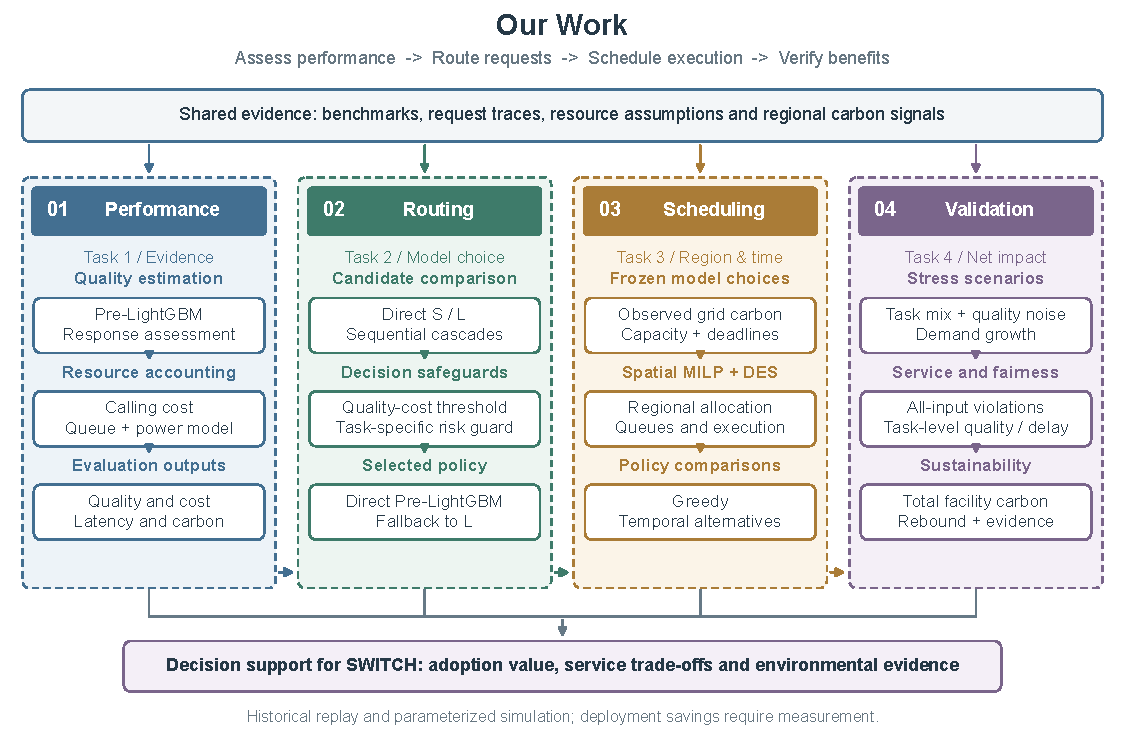
\includegraphics[width=\linewidth]{figures/B_four_column_framework.pdf}
  \caption{Overview of our framework: performance evaluation, protected model routing, carbon-aware scheduling, and robustness and sustainability assessment.}
  \label{fig:our-work}
\end{figure}
